\section{对数与对数函数}
\subsection{对数的概念与运算}
在讲什么是对数之前，应该说说什么是“逆运算”。所谓逆运算\footnote{也可以认为是为了“撤销”某个操作而产生的运算}，就是在反求“参与运算的量”的一种运算方式.
其实我们已经见过很多逆运算的例子了，比如加法和减法互为逆运算，
\[\text{加数+加数=和}\]
\[\text{被减数—减数=差}\]
乘法和除法互为逆运算。
\[\text{乘数}\times \text{乘数=积}\]
\[\text{被除数}\div\text{除数=商} \]

注意，加法的逆运算减法是唯一的，因为两个加数的地位是相等的（换言之，加法是有交换律的）；同样，减法的逆运算除法也是如此也是。

而对于幂运算，情况完全一样吗？

我们就知道“平方”与“开方”互为逆运算，即我们面对形如
\[x^2=a(x,a>0)\]的方程的时候，只要两侧开根号即可得\[x=\sqrt{a}\]
显然这个过程指数可以从$2$推广至任意的大于$1$的实数，而我们总是可以进行类似的操作根据幂和指数来求底数。
而我们知道，指数式由三部分组成：底数，指数，幂。底数和指数的地位并不相等，也就是说应该有一种运算是根据幂和底数来求指数。
而这种运算就是这节要介绍的求对数。
\begin{definition}[对数]
    \ 

    $\forall a>0\text{且}a\ne1,x\in \mathbb{R},\exists!N>0$，使得
    \[a^x=N\]

    则定义
    \[\log_aN:=x\]

    在对数式中，$a$称作底数，$N$称作真数，$\log_aN$称作对数，读作“以$a$为底$N$的对数”。
\end{definition}

\begin{minipage}{0.65\textwidth}

    一个自然的问题是：这样的定义出来的对数是唯一的吗？即对于给定的$a>0\text{且}a\neq1$和$N>0$，是否存在唯一的$x_0$
    使得$a^{x_0}=N$？答案是显然的，由于$f(x)=a^{x}$是严格单调的，其图像和水平直线$y=N$的交点是唯一的，
    而交点横坐标便是对应的$x_0$。（如右图）  
\end{minipage}%
\hfill%
\begin{minipage}{0.25\textwidth}
    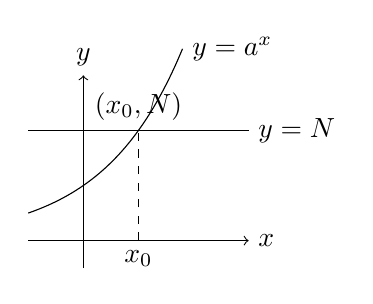
\begin{tikzpicture}[scale=0.7]
    % 绘制坐标轴
    \draw[->] (-1,0) -- (3,0) node[right] {$x$};
    \draw[->] (0,-0.5) -- (0,3) node[above] {$y$};
  
    % 绘制 y=2^x 曲线
    \draw[domain=-1:1.8,smooth,variable=\x] plot ({\x},{2^\x}) node[right] {$y=a^x$};
  
    % 绘制 y=2 直线
    \draw[smooth] (-1,2) -- (3,2) node[right] {$y=N$};
  
    % 标注交点和 (1,0)
    %\draw[dotted] (0,0) -- (1,0) node[below] {$1$};
    %\draw[dotted] (1,0) -- (1,{2^1}) node[midway,right] {$(1,2)$};
  
    % 连接交点和 (1,0) 的虚线
    \draw[dashed] (1,0) -- (1,{2^1});
  
    % 在 x 轴上方标注交点坐标
    \node[above] at (1,{2^1}) {$(x_0, N)$};
  
    % 在 x 轴下方标注 (1,0) 为 x_0
    \node[below] at (1,0) {$x_0$};
    \end{tikzpicture}
\end{minipage}

下面我们跟着定义来具体计算一些例子：
\begin{example}
    \ 

    $\log_24$

    $\log_2\frac{1}{2}$
\end{example}
在上面那个例子中我们注意到了形如
\begin{theorem}[对数恒等式]
    
\end{theorem}
\begin{example}
    $4^{\log_4 3}$
\end{example}
在实际使用中，有两种常用的对数——常用对数和自然对数。
\begin{definition}[自然对数与常用对数]
    

    \[\e:=\lim_{n\rightarrow +\infty}(1+\frac{1}{n})^n
    =\sum_{n=1}^{+\infty}\frac{1}{n!}\]
    \[\ln x \coloneqq \log _e x\]
    \[\lg x \coloneqq \log _{10} x\]
    $\lg(3x+2)$
\end{definition}

当然，以哪种对数为底并不是很重要
\begin{theorem}[换底公式]
    \[\log_a b=\frac{\log_c b}{\log_c a}\]
\end{theorem}
\begin{proof}
    
\end{proof}

\begin{theorem}[对数的运算法则]
    \ 

    $\forall M,N>0,a>0$且$a\ne1,n\in\mathbb{R}$，有
    \[\log_aN+\log_aM=\log_aMN\]
    \[\log_aM-\log_aN=\log_a\frac{M}{N}\]
    \[\log_aM^n=n\log_aM\]
\end{theorem}
\begin{proof}
    

    \qed
\end{proof}
\begin{example}[对数表的应用]
    
\end{example}
\begin{example}
    
\end{example}

\begin{corollary}
    
\end{corollary}
\clearpage
\subsection{对数函数}

\clearpage

\hw
% 第三题：零点结论判断（填空题）
\begin{homework}
已知函数 \( f(x) = \ln \dfrac{1 + x}{1 - x} \), 则

% Long options: split into two rows for each option (using fixed-width columns for text wrapping)
\begin{table}[H]
  \begin{tabular}{lp{0.7\textwidth}}
    \text{A.} & \( f(x) \) 在 \((-1,1)\) 上是减函数, 且曲线 \(y = f(x)\) 存在对称轴 \\ 
    \text{B.} & \( f(x) \) 在 \((-1,1)\) 上是减函数, 且曲线 \(y = f(x)\) 存在对称中心 \\ 
    \text{C.} & \( f(x) \) 在 \((-1,1)\) 上是增函数, 且曲线 \(y = f(x)\) 存在对称轴 \\ 
    \text{D.} & \( f(x) \) 在 \((-1,1)\) 上是增函数, 且曲线 \(y = f(x)\) 存在对称中心 \\ 
  \end{tabular}
\end{table}
\end{homework}
\begin{homework}
已知函数 \( f(x) = |\lg x| - kx - 2 \), 给出下列四个结论：
\begin{enumerate}
  \item 若 \( k=0 \), \( f(x) \) 恰有 2 个零点; 
  \item 存在负数 \( k \), 使得 \( f(x) \) 恰有 1 个零点; 
  \item 存在负数 \( k \), 使得 \( f(x) \) 恰有 3 个零点; 
  \item 存在正数 \( k \), 使得 \( f(x) \) 恰有 3 个零点.
\end{enumerate}
其中所有正确结论的序号是\underline{\hspace{2cm}}.
\end{homework}